\documentclass[10pt,landscape]{scrartcl}
\usepackage{multicol}
\usepackage{calc}
\usepackage{ifthen}
\usepackage[landscape]{geometry}
% Umlaute ermöglichen
\usepackage[T1]{fontenc}
% Format dieses Dokuments
\usepackage[utf8]{inputenc}
% Deutsche Trennungsregeln
\usepackage[ngerman]{babel}
\usepackage[babel,german=quotes]{csquotes}
\usepackage{listings}
\lstset{emph={%  
    wiederhole, bis, solange, setze, gebe%
    },emphstyle={\bfseries}%
}
%%\usepackage{color}
%\definecolor{lightgrey}{gray}{0.75}
%\definecolor{darkgrey}{gray}{0.25}

\usepackage{amssymb,amsmath}

\usepackage{tikz}
\usetikzlibrary{arrows,automata}

\usepackage{ulem}

\usepackage{hyperref}
%\pdfoutput=1
\hypersetup{
	pdfauthor   = {Lazari, Constantin},
	pdftitle    = {Informatik Cheat Sheet (1/4)},
	pdfsubject  = {Informatik},
	pdfkeywords = {},
	pdfcreator  = {Kile},		% Texnic Center oder Kile z.B.
	pdfproducer = {pdflatex},
	colorlinks  = false		% Links nicht farbig hervorheben (sieht Scheisse aus).
} 

% To make this come out properly in landscape mode, do one of the following
% 1.
%  pdflatex latexsheet.tex
%
% 2.
%  latex latexsheet.tex
%  dvips -P pdf  -t landscape latexsheet.dvi
%  ps2pdf latexsheet.ps

% This sets page margins to .5 inch if using letter paper, and to 1cm
% if using A4 paper. (This probably isn't strictly necessary.)
% If using another size paper, use default 1cm margins.
\ifthenelse{\lengthtest { \paperwidth = 11in}}
	{ \geometry{top=.5in,left=.5in,right=.5in,bottom=.5in} }
	{\ifthenelse{ \lengthtest{ \paperwidth = 297mm}}
		{\geometry{top=1cm,left=1cm,right=1cm,bottom=1cm} }
		{\geometry{top=1cm,left=1cm,right=1cm,bottom=1cm} }
	}

% Turn off header and footer
\pagestyle{empty}
 
% Redefine section commands to use less space
\makeatletter
\renewcommand{\section}{\@startsection{section}{1}{0mm}%
                                {-1ex plus -.5ex minus -.2ex}%
                                {0.5ex plus .2ex}%x
                                {\normalfont\large\bfseries}}
\renewcommand{\subsection}{\@startsection{subsection}{2}{0mm}%
                                {-1explus -.5ex minus -.2ex}%
                                {0.5ex plus .2ex}%
                                {\normalfont\normalsize\bfseries}}
\renewcommand{\subsubsection}{\@startsection{subsubsection}{3}{0mm}%
                                {-1ex plus -.5ex minus -.2ex}%
                                {1ex plus .2ex}%
                                {\normalfont\small\bfseries}}
\newcommand{\msout}[1]{\text{\sout{\ensuremath{#1}}}}
\makeatother

% Define BibTeX command
\def\BibTeX{{\rm B\kern-.05em{\sc i\kern-.025em b}\kern-.08em
    T\kern-.1667em\lower.7ex\hbox{E}\kern-.125emX}}

% Don't print section numbers
\setcounter{secnumdepth}{0}
\setlength{\parindent}{0pt}

\setlength{\parskip}{0pt plus 0.5ex}


% -----------------------------------------------------------------------

\begin{document}

	\raggedright
	\footnotesize
	\begin{multicols}{3}


	% multicol parameters
	% These lengths are set only within the two main columns
	%\setlength{\columnseprule}{0.25pt}
	\setlength{\premulticols}{1pt}
	\setlength{\postmulticols}{1pt}
	\setlength{\multicolsep}{1pt}
	\setlength{\columnsep}{2pt}
	\newlength{\MyLenA}
	\newlength{\MyLenB}

	\begin{center}
	\Large{\textbf{Informatik Cheat Sheet}} \\
	\end{center}

	Informatik ist die Wissenschaft der systematischen Verarbeitung von Informationen, insbesondere der automatisierten Verarbeitung durch Rechenanlagen.

\settowidth{\MyLenA}{Theoretische I.~~}
\begin{tabular}{@{}p{\the\MyLenA}%
				@{}p{\linewidth-\the\MyLenA}}
Theoretische I. & Algorithmen, Leistungsfähigkeit derselben, Entscheidbarkeit \dots\\
Praktische I.	& Software, Konzepte zur Organisation und Verwaltung von Daten\\
Technische I.	& Hardware, elektronischer Datenaustausch\\
Angewandte I.	& Einsatz von Informatik in anderen Disziplinen (Wirtschaft, Medizin \dots)\\
\end{tabular}

	\section{Geschichte}

\subsection{Grundlagen}
\subsubsection{Theorie}
\settowidth{\MyLenA}{Entscheidbarkeitsprobleme (1931)~~}
\begin{tabular}{@{}p{\the\MyLenA}%
				@{}p{\linewidth-\the\MyLenA}}
	Rechengesetze (15. Jh.) & Adam Ries\\
	Binäre Zahlendarstellung (1703) & Gottfried Leibniz\\
	Boolesche Algebra (1847)	& George Boole\\
	Entscheidbarkeitsprobleme (1931) & Kurt Gödel\\
	Turingmaschine (1936)	& Alan Turing\\
	Von-Neumann-Architektur & John v. Neumann\\
\end{tabular}

\subsubsection{Technik}
\settowidth{\MyLenA}{Programmiersprache Fortran (1955)~~}
\begin{tabular}{@{}p{\the\MyLenA}%
				@{}p{\linewidth-\the\MyLenA}}
	Bipolartransistor (1947) & Bell Laboratories\\
	Programmiersprache Fortran (1955) & IBM\\
	Chomsky-Hierarchie	(1956) & Noam Chomsky\\
	Unix (1969) & Bell Laboratories\\
\end{tabular}

\subsection{Generationen}
\settowidth{\MyLenA}{Generation 5 (seit 1992)~~}
\begin{tabular}{@{}p{\the\MyLenA}%
				@{}p{\linewidth-\the\MyLenA}}
Generation -1 (-1886) & Mechanische Rechmaschinen (Abakus, \dots, Lochkartengesteuerten Zählmaschine)\\
Generation 0 (-1943) & Elektro-mechanische Rechenmaschinen (Z1-Z3)\\
Generation 1 (-1950) & Elektronische Rechner mit Röhren (Eniac, Z4)\\
Generation 2 (-1960) & Elektronische Rechner mit Transistoren (TRADC)\\
Generation 3 (-1968) & Rechner mit integrierten Schaltkreisen (Texas Instruments)\\
Generation 4 (-1984) & Hochintegrierte Computer (IBM-PC, Macintosh)\\
Generation 5 (seit 1992) & Vernetzte und parallele Computer (8 Petaflops mit 80\,000 8-Kern Prozessoren)\\
\end{tabular}

\subsection{Mooresches Gesetz}
\enquote{Die Komplexität integrierter Schaltkreise mit minimalen Komponentenkosten verdoppelt sich regelmässig.}
Etwa alle 20 Monate verdoppelt sich die Anzahl Transistoren pro Fläche. Speicherkarten werden günstiger.

% \subsection{Von-Neumann-Architektur}
% 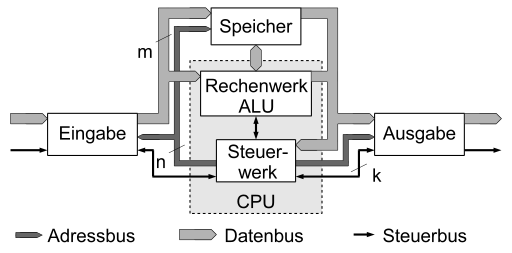
\includegraphics[width=\linewidth]{von_Neumann-_Architektur_de.png}
% \subsubsection{Unterschied zur Harvard-Archiktektur}
% Die Harvard-Architektur trennt zusätzlich den Arbeits- bzw. Datenspeicher physisch vom
% Programmspeicher.

\subsection{Grössenangaben}
\begin{tabular}{c|c|c|c|}
	\textbf{Metrisch} & \textbf{Anzahl} & \textbf{Binärpräfix} & \textbf{Anzahl}\\
	\hline
	Kilobyte [kB] & $10^{3}$ Byte & Kibibyte [KiB] & $2^{10}$ Byte \\
	Megabyte [MB] & $10^{6}$ Byte & Mebibyte [MiB] & $2^{20}$ Byte \\\hline
	Gigabyte [GB] & $10^{9}$ Byte & Gibibyte [GiB] & $2^{30}$ Byte \\
	Terabyte [TB] & $10^{12}$ Byte & Tebibyte [TiB] & $2^{40}$ Byte \\\hline
	Petabyte [PB] & $10^{15}$ Byte & Pebibyte [PiB] & $2^{50}$ Byte \\
	Exabyte [EB] & $10^{18}$ Byte & Exbibyte [EiB] & $2^{60}$ Byte \\\hline
	Zetabyte [ZB] & $10^{21}$ Byte & Zebibyte [ZiB] & $2^{70}$ Byte \\
	Yotabyte [YB] & $10^{24}$ Byte & Yobibyte [YiB] & $2^{80}$ Byte \\
\end{tabular}\\
iB zu B: Exponent = $\log_{2}$ Bytes

	\section{Begriffe}
\begin{description}
 \item [Information] (lat. \enquote{informatio}, Form oder Gestalt geben) ist nicht einheitlich
 definiert. Im allgemeinen wird darunter \enquote{übertragenes Wissen} verstanden.
 \item [Daten] (lat. \enquote{datum}, gegebenes) ebenfalls nicht einheitlich definiert. Grundsätzlich
 codierbare Angaben über Dinge oder Sachverhalte, die gespeichert und verarbeitet werden können.
 Die jährlich produzierte Datenmenge liegt bei ca. 10 Zettabytes ($10^{21}$ Bytes)
 \item [strukturierte Daten] haben eine explizite Struktur und sind in der Minderheit (Bsp. Tabellen)
 \item [unstruktierte Daten] haben keine explizite Struktur (ggf. implizite Struktur aufgrund einer
 zugrunde liegenden Grammatik. (Bsp. Text, Bilder, Filme, \dots)
 \item [semistrukturierte Daten] sind nur zum Teil strukturiert (Bsp. XML)
\end{description}

\subsection{Dateisystem vs. DBMS}
\subsubsection{Dateisystem}
Daten werden in Dateien vom Betriebssystem verwaltet. Anwendungen lesen/schreiben die Daten direkt. (Office-Anwendungen,
Buchhaltungssoftware, \dots)


% \begin{tabular}{
% 	@{}p{\linewidth/2}|
% 	@{}p{\linewidth/2}}
% 	\multicolumn{1}{c}{Vorteile} & \multicolumn{1}{c}{Nachteile}\\
% 	\begin{minipage}{\linewidth}
		\begin{itemize}
			\item [$+$] einfach, angepasst, effizient
			\item [$+$] keine Rücksicht auf andere
			\item [$+$] proprietäre Formate möglich
% 		\end{itemize}
% 	\end{minipage}
% 	&
% 	\begin{minipage}{\linewidth}
% 		\begin{itemize}
			\item [$-$] Verwendung für unterschiedliche Zwecke problematisch
			\item [$-$] i.d.R. Strukturänderung $\Rightarrow$ Programmänderung 
			\item [$-$] Synchroner Zugriff aufwändig zu realisieren
			\item [$-$] Abgestufte Zugriffsrechte aufwänding zu realisieren
			\item [$-$] Daten häufig mehrfach gespeichert
			\item [$-$] Datenaustausch, -integration komplex
		\end{itemize}
% 	\end{minipage}	
% \end{tabular}

\subsubsection{Datenbanksysteme}
Verwalten und nutzen (sehr) grosse Datenmengen. Der Zugriff ist deklarativ und mengenorientiert.
Die Daten werden einmalig und zentral definiert. Wichtige Aufgaben (Integritätskontrolle, Redundanzverwaltung,
Zugriffskontrolle und -optimierung, synchroner Zugriff, zentrale Datensicherung und Wiederherstellung) 
können so automatisiert werden. Allerdings sind Aufbau und Betrieb eines Datenbanksystems anspruchsvoll und teuer.


\subsection{Datenunabhängigkeit (DU)}
\begin{description}
	\item [Logische DU] Anwendungsprogramme müssen die logische Gesamtstruktur nicht kennen,
	um spezifische Verarbeitungen vorzunehmen $\Rightarrow$ sie sind von Datenbankschema-Änderungen
	nicht betroffen.
	\item [Physische DU] Anwendungsprogramme müssen die interne Organisation der Daten und Zugriffs- 
	und Speicherungsmöglichkeiten nicht kennen $\Rightarrow$ sie sind von Speicher- und Zugriffstrukturänderungen
	nicht betroffen
\end{description}

\subsection{Datenbank Management Systeme}
\textbf{DB-Typen:} hierarchisch, relational, objekt-relational, objektorientiert, deduktiv, netzwerk, \dots

Ein Datenbanksystem (DBS) besteht aus einem Datenbankverwaltungssystem (Software, DBMS) und einer Datenbank (Daten, DB).
Anwendungsprogramme kommunizieren mit dem DBMS. Anwendungsprogramme und DBS bilden ein Informationssystem (IS).

\subsubsection{Aufgaben DBMS}
Syntaxprüfung, Objekte und Zugriffsrechte prüfen, Metadaten lesen, Zugriffsmodul generieren, Transaktionskontrolle,
Daten lesen, Daten zusammenstellen, Daten ausgeben.

% \begin{tabular}{@{}p{\linewidth/2}|@{}p{\linewidth/2}}
%  \multicolumn{1}{c}{Dateisystem} & \multicolumn{1}{c}{Datenbank} \\\hline
%  + einfach, anpassbar, effizient & + langfristige Aufbewahrung\\
%  + Proprietäre Formate möglich & + grosse Mengen\\
%  + Keine Rücksicht auf ander & + viele Benutzer\\
%  - Struktur = Programmänderung & + einfache Rechteverwaltung\\
%  - Simultaner Zugriff schwierig & + logische Unabhängigkeit\\
%  - abgest. Zugriffsrechte schwierig & + physische Unabhängigkeit\\
%  - Mehrfachverwendung heikel &  + Automatisierung\\
%  - Logische \& physische abhängig & - teuer und aufwändig\\
% \end{tabular}

\subsubsection{ANSI-SPARC-3-Ebenen-Architektur (1975)}
\begin{description}
 \item [Extern] Sicht einzelner Anwendungen oder Benutzergruppen
 \item [Konzeptionell] Logische Gesamtsicht
 \item [Intern] Speicherung, Datenorganisation, Zugriffsstrukturen
\end{description}

\subsubsection{Aufbau und Betrieb}
Auf- und Ausbau bezeichnet das (iterative) erstellen verschiedener Datenbank Schemas, 
häufig im laufenden Betrieb. Betrieb, Nutzung und Verwaltung (Anzeigen, Einfügen, Ändern, Löschen, Backup, Restore)
mit Hilfe der Daten-Manipulationssprache (DML)

	\section{Zahlensysteme}

\subsection{Darstellung allgemein}
Jede gebrochene Zahl $z$ mit $n$-Stellen vor und $m$ Stellen nach dem Komma ($n, m \in \mathbb{N}\textbackslash\{0\}$) 
mit einer Basis $B$ und den Ziffern $b \in \{0, 1, \dots, B-1\}$ lässt sich als Summe darstellen:
\begin{equation*}
	z = \sum_{i=-m}^{n-1} b_i \cdot B^i
\end{equation*}

\subsection{Konvertierung}
\subsubsection{Zahlensystem zur Basis $B$ ins Dezimalsystem}
$n$ = Vorkommastellen, $m$ = Nachkommastellen
\settowidth{\MyLenA}{Nach~~}
\begin{tabular}{@{}p{\the\MyLenA}%
				@{}p{\linewidth-\the\MyLenA}}
	Vor  & $z = (\dots((b_n \cdot B + b_{n-1}) \cdot B + b_{n-2}) \cdot B + \dots + b_1) \cdot B + b_0$\\
	Nach  & $z = (\dots((b_m \cdot 1/B + b_{-m+1}) \cdot 1/B + b_{-m+2}) \cdot 1/B + \dots + b_{-1}) \cdot 1/B$\\
\end{tabular}

\subsubsection{Dezimalsystem in System zur Basis $B$}

\textbf{Vorkommastellen} Eingabe Vorkommastellen $n$, Basis $B$\\
Wiederhole
\begin{enumerate}
	\item $y = n : B$ Rest $z$ (Dividiere durch $B$, behalte $z$)
	\item $n = y$ (Rechne mit Divisionsergebnis ohne Rest weiter)
\end{enumerate}
bis ($y = 0)$\\
Die Reste $z$ von unten nach oben ergeben die die gesuchte Zahl.

Beispiel: $n = 122$, gesucht Darstellung zur Basis 8 (Oktal)
\begin{align*}
	122 \div 8 = 15&~\mbox{Rest}~2\\
	15 \div 8 = 1&~\mbox{Rest}~7\\
	1 \div 8 = 0&~\mbox{Rest}~1 \rightarrow 122_{10} = 172_8
\end{align*}

\textbf{Nachkommastellen} Eingabe Nachkommastellen $m$, Basis $B$\\
Wiederhole
\begin{enumerate}
	\item $y = m \cdot B$ (Multipliziere $m$ mit $B$)
	\item $m = \mbox{frac}(y)$ (Setze den Nachkommateil von $y$ zum neuen $m$)
\end{enumerate}
bis ($m = 0$)\\
Die ganzzahligen Anteile von oben nach unten ergeben die gesuchte Zahl.

Beispiel: $n = 0{,}3984375$, gesucht Darstellung zur Basis 8 (Oktal)
\begin{align*}
	0{,}3984375 \cdot 8 = 3{,}1875&~\mbox{Ganzzahlanteil:}~3\\
	0{,}1875 \cdot 8 = 1{,}5&~\mbox{Ganzzahlanteil:}~1\\
	0{,}5 \cdot 8 = 4{,}0&~\mbox{Ganzzahlanteil:}~4 \rightarrow 0{,}3984375_{10} = 0{,}314_8
\end{align*}

\subsection{Einerkomplement}
Erstes Bit = Vorzeichen (1 für negativ), Zahl = Invertierung der positiven Zahl.
Überlauf ist, wenn zu einer 1 ganz links, eine 1 addiert wird. Diese wird der Ziffer ganz rechts hinzugefügt.
Nachteile: Redundante Darstellung der 0, separate Betrachtung des Überlaufs $\rightarrow$ 2 Additionen

\subsection{Zweierkomplement}
Beim Zweierkomplement werden negativen Zahlen des Einerkomplements um 1 erhöht. Beim Überlauf wird ein 
Warnmeldungsflag (Overflow) auf wahr gesetzt.

\subsection{Festpunktzahlen}
Haben eine festgelegte Länge von Vorkommazahlen ($n$) und Nachkommazahlen ($m$).
Sie decken jeweils nur einen bestimmten Wertebereich ab, gewisse Zahlen lassen sich exakt darstellen, andere nicht.
Rechnen mit Werten sehr unterschiedlicher Grösse ist schwierig bis unmöglich. Festkommazahlen werden daher nur
für Spezialanwendungen gebraucht.

\subsection{Fliesskommazahlen}
(IEEE 754): $s$ = Vorzeichen (0 positiv, 1 negativ), $M$ = Mantisse, $B$ = Basis und $E$ = Exponent.
\begin{equation*}
x = s  \cdot B^E \cdot M
\end{equation*}
Die Mantisse ist 23 bzw. 52 Bit lang und sie ist normiert (Dargestellt als 1.xxx), wobei die führende 1 weggelassen wird 
um die Präzision um ein Bit zu erhöhen, also zu verdoppeln.

	\begin{tabular}{ll}
							& \textbf{Single Precision}\\ 
	Vorzeichen				& 1 Bit\\
	Exponent				& 8 Bit\\
	Mantisse				& 23 Bit\\
	Gesamtlänge				& 32 Bit\\
	Biaswert				& 127\\
	Wertebereich Exponent 	& $-126 \leq e \leq 127$\\
	Dezimalstellen 			& 7 \dots\ 8\\
	Genauigkeit				& $2^{-(23 + 1)} \approx 5{,}96 \cdot 10^{-8}$\\
	Minimum					& $2^{-(23 + 126)} \approx 1 \cdot 10^{-45}$\\
	Maximum					& $(1 - 2^{-24}) \cdot 2^{128} \approx 3{,}4 \cdot 10^{38}$\\
	\end{tabular}
	\begin{tabular}{ll}
							& \textbf{Double Precision} \\
	Vorzeichen				& 1 Bit	\\
	Exponent				& 11 Bit\\	
	Mantisse				& 52 Bit\\
	Gesamtlänge				& 64 Bit\\
	Biaswert				& 1\,023\\
	Wertebereich Exponent	& $-1\,022 \leq e \leq 1\,023$\\
	Dezimalstellen			& 15 \dots\ 16\\
	Genauigkeit				& $2^{-(52 + 1)} \approx 1{,}1\cdot 10^{16}$\\
	Minimum					& $2^{-(52 + 1\,022)} \approx 5 \cdot 10^{-324}$\\
	Maximum					& $(1 - 2^{-52}) \cdot 2^{1\,024} \approx 1{,}8 \cdot 10^{308}$\\
	\end{tabular}

Beispiel: Darstellung von $18{,}4_{10}$ als IEEE 754 Gleitpunktzahl:
\begin{enumerate}
	\item Vorzeichen: positiv $\rightarrow 0$ 
	\item Mantisse:
		\begin{enumerate}
			\item Umwandlung in duale Festkommazahl ohne Vorzeichen:
			\begin{align*}
				18_{10}& = 1\,0010_2\\
				0.4_{10}& = 0.01100\,\overline{1100}_2\\
				18.4_{10}& = 1\,0010.01100\overline{1100}_2
			\end{align*}
			\item Normalisierung
			\begin{equation*}
				18.4_{10} = 1\,0010.01100\,1100\,\dots_2 \cdot 2^0 = 
1.0010\,01100\,\overline{1100}_2 \cdot 2^4
			\end{equation*}
			Aus $2^4 \rightarrow e = 4$
		\end{enumerate}
	\item Exponent:
		\begin{enumerate}
			\item Exponent $e=4$, Biaswert = 127;
			\item $E = e + Biaswert = 4_{10} + 127_{10} = 131_{10} = 1000\,0011_2$
		\end{enumerate}
\end{enumerate}
Die zusammengesetzte Gleitpunktzahl ist: $0\,10000011\,00101100110011001100110$

	\section{Codierungen}
\subsection{ASCII (1963)}
ASCII steht für \enquote{American Standard Code for Information Interchange}, 7 Bit, 95 druckbare + 33 Steuerzeichen = 128 Zeichen.
\begin{center}
\begin{tabular}{c|c||c|c|c|c|c|c|c|c|}
			\multicolumn{2}{c||}{}  & \textbf{0} 	& \textbf{1} 	& \textbf{2} 	& \textbf{3}			& \textbf{4} 	& \textbf{5} 	& \textbf{6} 	&  \textbf{7}	\\\hline
\textbf{0}	& $0000_2$	&	NUL			& DLE			& SP			& 0				& @ 			& P				& `				& p				\\
\hline
\textbf{1}	& $0001_2$	& SOH			& DC1			& !				& 1				& A				& Q				& a				& q				\\
\hline
\textbf{2}	& $0010_2$	& STX			& DC2 			& "' 			& 2 			& B				& R 			& b 			& r 			\\
\hline
\textbf{3}	& $0011_2$	& ETX 			& DC3 			& \# 			& 3 			& C 			& S 			& c 			& s 			\\
\hline
\textbf{4}	& $0100_2$ 	& EOT 			& DC4 			& \$ 			& 4 			& D 			& T 			& d 			& t 			\\
\hline
\textbf{5}	& $0101_2$	& ENQ 			& NAK 			& \% 			& 5 			& E 			& U 			& e 			& u 			\\
\hline
\textbf{6}	& $0110_2$ 	& ACK 			& SYN 			& \& 			& 6 			& F 			& V 			& f 			& v 			\\
\hline
\textbf{7} 	& $0111_2$	& BEL 			& ETB 			& ' 			& 7 			& G 			& W 			& g 			& w 			\\
\hline
\textbf{8} 	& $1000_2$	& BS 			& CAN 			& ( 			& 8 			& H 			& X 			& h 			& x 			\\
\hline
\textbf{9} 	& $1001_2$	& TAB 			& EM 			& ) 			& 9 			& I 			& Y 			& i 			& y 			\\
\hline
\textbf{A} 	& $1010_2$	& LF 			& SUB 			& * 			& : 			& J 			& Z 			& j 			& z 			\\
\hline
\textbf{B} 	& $1011_2$	& VT 			& ESC 			& + 			& ; 			& K 			& [ 			& k 			& \{ 			\\
\hline
\textbf{C} 	& $1100_2$	& FF 			& FS 			& , 			& < 			& L 			& \textbackslash& l 			& $\mid$ 		\\
\hline
\textbf{D} 	& $1101_2$	& CR 			& GS 			& - 			& = 			& M 			& ] 			& m 			& \} 			\\
\hline
\textbf{E} 	& $1110_2$	& SO 			& RS 			& . 			& > 			& N 			& \^{} 			& n 			& "~ 			\\
\hline
\textbf{F} 	& $1111_2$	& SI 			& US 			& / 			& ? 			& O 			& \_ 			& o 			& DEL 			\\
\end{tabular}	
\end{center}

Beispiel Zeichen \enquote{j} = 6A

\subsection{ISO 8859}
8 Bit Erweiterung von ASCII. ISO 8859-1 = LATIN-1 (Europa). Aufbau:
\settowidth{\MyLenA}{Position 160 ($A0_{16}$) -- 255 ($FF_{16}$)~~}
\begin{tabular}{@{}p{\the\MyLenA}%
				@{}p{\linewidth-\the\MyLenA}}
	Position 0 ($00_{16}$) -- 127 ($7F_{16}$) & ASCII\\
	Position 128 ($80_{16}$) -- 159 ($9F_{16}$) & Steuerzeichen\\
	Position 160 ($A0_{16}$) -- 255 ($FF_{16}$) & regionale Sonderzeichen\\
\end{tabular}

\subsection{Unicode (1991)}
Zeichensatz bestehend aus 17 Bereiche zu je 65\,536 Zeichen.

\subsubsection{UTF-8}
UTF-8 ist eine Codierungsform für Unicode, die 1 bis 4 Bytes verwendet:
\settowidth{\MyLenA}{Form 0xxx\,xxxx~~}
\begin{tabular}{@{}p{\the\MyLenA}%
				@{}p{\linewidth-\the\MyLenA}}
	Form 0xxx\,xxxx & 1 Byte, codiert ist der ASCII Zeichensatz (128)\\
	Form 110x\,xxxx & 2 Byte, häufige Sonderzeichen ($2^{5+6} = 2\,048$)\\
	Form 1110\,xxxx & 3 Byte, weniger häufige Zeichen($2^{4+6+6} = 65\,536$)\\
	Form 1111\,0xxx & 4 Byte, selten Zeichen ($2^{3+6+6+6} = 2\,097\,152$)\\
	Form 10xx\,xxxx & Folgebyte\\
\end{tabular}
Jedes Zeichen, das mit mehr als einem Byte codiert ist, wird hat so viele Folgebytes, wie es selbst lang ist. (Bsp. 1110\,xxxx~10xx\,xxxx~10xx\,xxxx)

UTF-16 und UTF-32 verwenden für jedes Zeichen 2 respektive 4 Bytes.

	\subsection{Kompression}
\settowidth{\MyLenA}{Hamming-Abstand~~}
\begin{tabular}{@{}p{\the\MyLenA}%
				@{}p{\linewidth-\the\MyLenA}}
	Präfixfreiheit & Kein Wort ist der Anfang eines anderen Wortes (Fano-Bedingung)\\
	Zyklisch & Wenn aus einem Code-Wort alle anderen gültigen Code-Wörter abgeleitet werden können. (Bsp: abc, bca, cab)\\
	Hamming-Abstand & Anzahl unterschiedlicher Zeichen zweier gleichlanger Wörter\\
	Hamming-Distanz & Minimum des Hamming-Abstandes aller Wörter eines Codes\\
	Gray-Code		& Benachbarte Wörter haben den Hamming-Abstand 1\\
	Gleichverteilung & Alle Wörter gleich $n$ Bits lang: $\lceil n\rceil = \log_2 |Z|$\\
\end{tabular}

Umwandlung einer Dezimalzahl ($d$) in Graycode:
\begin{enumerate}
	\item Setze $s$ = Rechts-Shift von dezimal um 1 Bit
	\item Setze $g$ = XOR($d$, $s$)
	\item Gebe $g$ zurück
\end{enumerate}

\subsection{Shannon-Fano-Algorithmus}
Betrachte alle Zeichen als eine Gruppe.\\
Erstelle einen neuen Knoten auf der aktuellen Ebene.\\
Solange (Die Gruppe aus mehr als einem Zeichen besteht):
\begin{enumerate}
	\item Sortiere die Zeichen nach ihrer Häufigkeit.
	\item Teile die Zeichen entlang dieser Reihenfolge so in 2 Gruppen, dass die Summe der Häufigkeiten in den beiden Gruppen möglichst gleich ist.
	\item Führe diesen Algorithmus mit jeder Gruppe aus.
\end{enumerate}
Das Ergebnis weisst eine unnötig hohe Redundanz auf ($R = \frac{\mbox{mittlere Länge}}{\mbox{Entropie}} - 1$).
Die Anzahl der Ebenen unterhalb der Wurzel, gibt die Anzahl zu verwendender Bits an.

\subsection{Huffmann-Algorithmus}
Erstelle eine Wald mit einem Baum für jedes Zeichen.\\
Jeder dieser Bäume enthält nur einen einzigen Knoten: das Zeichen.\\ 
Schreibe die Häufigkeit an die Kante.\\
Wiederhole:
\begin{enumerate}
	\item Suche die beiden Bäume, die die geringste Häufigkeit haben.
	\item Fasse beide Bäume zusammen, indem sie die Teilbäume einer neuen Wurzel werden.
	\item Benutze die Summe der Häufigkeiten dieses neuen Baumes zur weiteren Analyse.
\end{enumerate}
bis nur noch ein Baum übrig ist.\\
Die Anzahl der Ebenen unterhalb der Wurzel, gibt die Anzahl zu verwendender Bits an.

\subsection{Arithmetische Codierung}
Kodierer und Dekodierer einigen sich auf ein Intervall. Normalerweise wird hier das halboffene Intervall $[0,1)$ verwendet.
Kodierer und Dekodierer bei der De- bzw. Kodierung eines Zeichens immer identische Tabellen 
Wahrscheinlichkeitstabellen aller dekodierbaren Zeichen. Der Algorithmus für die Codierung sieht dann wie folgt aus:
\begin{enumerate}
	\item Initialisiere das aktuelle Intervall mit dem vereinbarten Startintervall
	\item Zerlege das aktuelle Intervall auf die identische Art wie der Dekodierer in Subintervalle, 
		und weise jedem Subintervall ein Zeichen zu.
	\item Das Subintervall, das dem nächsten Zeichen der Eingabe entspricht, wird zum aktuellen Intervall.
	\item Sind noch weitere Zeichen zu kodieren, dann weiter bei Punkt 2. Sonst weiter beim nächsten Punkt.
	\item Gib eine beliebige Zahl aus dem aktuellen Intervall und zusätzlich die Anzahl der kodierten Zeichen aus. 
	Dieses ist die Zahl $x$, die vom Dekodierer wie oben beschrieben entschlüsselt werden kann. 
	Diese Zahl wird so gewählt, dass sie möglichst wenig Nachkommastellen hat, also möglichst „rund“ ist 
	und sich daher mit relativ wenigen Bits darstellen lässt.
\end{enumerate}

Beispiel: Gegeben sei das Wort \enquote{bad}.\\
\begin{tabular}{lclcl}
	$p(a) = 0{,}65$ & ~ & 
	$p(b) = 0{,}15$ & ~ &
	$p(c) = 0{,}10$ \\
	$p(d) = 0{,}04$ & ~ & 
	$p(e) = 0{,}04$ & ~ &
	$p(f) = 0{,}02$ 
\end{tabular}
\begin{enumerate}
	\item Startintervall sei $I_0 = [0, 1)$.
	\item Aufgrund der Häufigkeiten gelten folgende Teil-Intervalle:\\
		\begin{tabular}{lll}
			$I_a = [0, 0{,}65)$  & $I_b = [0{,}65, 0{,}80)$  & $I_c = [0{,}80, 0{,}90)$ \\
			$I_d = [0{,}90, 0{,}94)$  & $I_e = [0{,}94, 0{,}98)$  & $I_f = [0{,}98, 1{,}0)$ \\			
		\end{tabular}
	\item Erstes Zeichen = $b \rightarrow $ neues Startintervall = $I_0 = [0{,}65, 0{,}80)$
	\item Aufgrund der Häufigkeiten gelten folgende Teil-Intervalle:\\
		\begin{tabular}{lll}
			$I_a = [0{,}65, 0{,}7475)$  & $I_b = [0{,}7475, 0{,}77)$  & $I_c = [0{,}77, 0{,}785)$ \\
			$I_d = [0{,}785, 0{,}791)$  & $I_e = [0{,}791, 0{,}797)$  & $I_f = [0{,}797, 0{,}80)$ \\			
		\end{tabular}
	\item Zweites Zeichen = $a \rightarrow$ neues Startintervall = $I_0 = [0{,}65, 0{,}7475)$
	\item Aufgrund der Häufigkeiten gelten folgende Teil-Intervalle:\\
		\begin{tabular}{ll}
			$I_a = [0{,}65, 0{,}713375)$  & $I_b = [0{,}713375, 0{,}728)$\\  
			$I_c = [0{,}728, 0{,}73775)$  & $I_d = [0{,}73775, 0{,}74165)$\\
			$I_e = [0{,}74165, 0{,}74555)$  & $I_f = [0{,}74555, 0{,}7475)$ \\			
		\end{tabular}
	\item Drittes Zeichen = $d \rightarrow $ neues Startintervall = $[0{,}73775, 0{,}74165)$
	\item Da keine weiteren Zeichen vorhanden sind, eine möglichst kleine Zahl aus $[0{,}73775, 0{,}74165)$ wählen: $0{,}74 = \frac{74}{100}$
\end{enumerate}

Dekodierung:
Beispiel: Gegeben sei die Zahl $0{,}74$ für ein Wort bestehend aus drei Zeichen. Welches Wort verbirgt sich darin?
\begin{enumerate}
	\item Startintervall sei $I_0 = [0, 1)$.
	\item Aufgrund der Häufigkeiten gelten folgende Teil-Intervalle:\\
		\begin{tabular}{lll}
			$I_a = [0, 0{,}65)$  & $I_b = [0{,}65, 0{,}80)$  & $I_c = [0{,}80, 0{,}90)$ \\
			$I_d = [0{,}90, 0{,}94)$ & $I_e = [0{,}94, 0{,}98)$ & $I_f = [0{,}98, 1{,}0)$ \\			
		\end{tabular}
	\item $0{,}74$ liegt im Teil-Intervall von $I_b = [0{,}65, 0{,}80) \rightarrow$ das erste Zeichen ist ein $b$.
	\item Aufgrund der Häufigkeiten gelten folgende Teil-Intervalle:\\
		\begin{tabular}{lll}
			$I_a = [0{,}65, 0{,}7475)$ & $I_b = [0{,}7475, 0{,}77)$ & $I_c = [0{,}77, 0{,}785)$ \\
			$I_d = [0{,}785, 0{,}791)$ & $I_e = [0{,}791, 0{,}797)$ & $I_f = [0{,}797, 0{,}80)$ \\			
		\end{tabular}
	\item $0{,}74$ liegt im Teil-Intervall von $I_a = [0{,}65, 0{,}7475) \rightarrow$ das zweite Zeichen ist ein $a$.
	\item Aufgrund der Häufigkeiten gelten folgende Teil-Intervalle:\\
		\begin{tabular}{ll}
			$I_a = [0{,}65, 0{,}713375)$ & $I_b = [0{,}713375, 0{,}728)$\\
			$I_c = [0{,}728, 0{,}73775)$ & $I_d = [0{,}73775, 0{,}74165)$ \\
			$I_e = [0{,}74165, 0{,}74555)$ & $I_f = [0{,}74555, 0{,}7475)$ \\			
		\end{tabular}
	\item $0{,}74$ liegt im Teil-Intervall von $I_d = [0{,}73775, 0{,}74165) \rightarrow$ das dritte Zeichen ist ein $d$.
	\item Das gesuchte Wort ist \enquote{bad}
\end{enumerate}
Die Länge des gesuchten Wortes muss bekannt sein!


	\section{Fehler}
\settowidth{\MyLenA}{Synchronistationsfehler~~}
\begin{tabular}{@{}p{\the\MyLenA}%
				@{}p{\linewidth-\the\MyLenA}}
	Fehler & Ein Fehler liegt vor, wenn sich die gesendeten und empfangen bzw. abgespeicherte und ausgelesene $n$-Bits
	an mindestens einer Stelle unterscheiden (Bitweises XOR $\neq$ 0)\\
	Mehrfachfehler & Ein Mehrfachfehler von $x$-Bit liegt vor, wenn sich die gesendeten und empfangenen bzw. diesem
	abgespeicherten und ausgelesenen $n$-Bits an mindestens $x, x > 1$ Stellen unterscheiden.\\
	Einzelbitfehler & statistisch voneinander unabhängig -- das Auftreten eines Fehlers hängt nicht von
	anderen Fehlern ab.\\
	Bündelfehler  & (Blockfehler, Bursts) mehrere direkt aufeinanderfolgende Bits fehlerhaft
	sind -- das Auftreten hängt von anderen/früheren Fehlern ab.\\
	Synchronistationsfehler & lange Bündelfehler
\end{tabular}

\subsection{Fehlerursachen}
Typische physikalische Ursachen für Fehler sind:
\begin {itemize}
	\item Rauschen (Wärme- oder Impulsrauschen) verursacht langfristig gleichmässig verteilte Einzelbitfehler. 
	\item Dämpfung, Dispersion (Aufgrund von Leitungswiderstand, Dämpfung, Reflexion) verusacht Einzelbitfehler oder Bündelfehler.
	\item Strahlung (kosmische, radioaktive) verusacht langfristig gleichmässig verteilte Einzelbitfehler. 
	\item Störungen (elektr. Funken, Kratzer) führen zu Bündelfehlern. Die Fehler sind ungleichmässig verteilt.
	\item Nebensprechen (kapazitive Kopplung benachbarter Datenleitungen) verursacht ungleichmässig verteilte Bündelfehler.
\end{itemize}

\subsection{Einfache Parität}
Die einfache Parität wird auch einfach gebildet:
\begin{enumerate}
	\item Die Code-Wörter werden um ein zusätzliches Bit, das Paritäts-Bit erweitert.
	\item Der Wert dieses Bits wird bei:
		\begin{description}
			\item [gerader Parität (even parity)] so gesetzt, dass die Summe der Einsen im Code-Wort inkl. des Paritäts-Bits gerade ist.
			(Beispiel: Das Code-Wort sei $0100.1110 \rightarrow $ 4 Einsen sind gerade $\implies$ Paritätsbit = 0) 
			\item [ungerader Parität (ungerade)] so gesetzt, dass die Summe der Einsen im Code-Wort inkl. des Paritäts-Bits ungerade ist.
			(Beispiel: Das Code-Wort sei $0100.1110 \rightarrow $ 4 Einsen sind gerade $\implies$ Paritätsbit = 1) 
		\end{description}
\end{enumerate}

\begin{itemize}
	\item Alle ungeraden-Bit-Fehler können erkannt werden
	\item Gerade-Bit-Fehler können nicht erkannt werden
	\item Bündelfehler können nur zu 50\% erkannt werden
	\item Fehler können nicht korrigiert werden.
\end{itemize}

\subsection{Zweidimensionale Parität}
Ansatz:
\begin{itemize}
	\item Ein Block-Code aus $n$-Bits wird in Wörter gleicher Länge $l$ aufgeteilt.
	\item Jedes Wort wird um ein Paritätsbit ergänzt
	\item Jedes $i$-te Bit (inkl. Paritätsbit) jedes Wortes wird ebenfalls um ein Paritätsbit ergänzt.
\end{itemize}

Im Ergebnis:
\begin{itemize}
	\item 1-Bit-Fehler werden doppelt erkannt (Zeile und Spalte) und können korrigiert werden
	\item ungerade-Bit-Fehler werden erkannt, können aber nicht korrigiert werden (Maskierung)
	\item 2, 6, 10, \dots-Bit-Fehler werden erkannt (Zeile oder Spalte), können aber nicht korrigiert werden
	\item Vielfache von 4-Bit-Fehler werden in aller Regel erkannt. Es sei denn, sie maskieren sich doppelt, was nur extrem selten 
	(Bsp. bei einer Anordnung im Viereck) der Fall ist
	\item Bündelfehler werden nur Ausnahmsweise nicht erkannt.
\end{itemize}

\subsection{Blockcode - CRC}
$(n, k)$-Block Code bedeutet, dass für $k$ übertragene Nutzdatenbits $n-k$ Prüfbits und somit insgesamt $n$-Bits übertragen werden.

\subsubsection{Algorithmus}
Eine Bitfolge von $n$-Bits wirt als Nachrichtenpolynom vom Grad $n-1$ dargestellt:
\begin{equation*}
 I(x) = a_{n-1}x^{n-1} + a_{n-2}x^{n-2} + \dots + a_1x^1 + a_0x^0 = \sum_{i=0}^{n-1} a_i \cdot x^i
\end{equation*}

Ein Generatorpolynom $C(x)$ mit Grad $n-k, n > k, n \in \mathbb{N}$ wird zwischen Sender und Empfänger
vereinbart.

Der genaue Algorithmus zur Übermittlung einer Nachricht $I(x)$ und dem Generatorpolynom $C(x)$ vom Grad $n-k$ 
liesst sich folgendermassen:
\begin{enumerate}
 \item Sender erzeugt $N(x)$:
    \begin{enumerate}
      \item $M(x) = I(x)\cdot x^{n-k}$
      \item $R_s(x) = I(x) \mod C(x)$
      \item $N(x) = (M(x) + R_s(x))$
    \end{enumerate}
  \item Sender sendet $N(x)$
  \item Empfänger berechnet: $R_e = N(x) \mod C(x)$ und entscheidet:
    \begin{itemize}
     \item Falls $R_e = 0$: Kein Fehler, also $I(x) = M(x) + R_s(x)$
     \item Falls $R_e \neq 0$: Ein Fehler ist aufgetreten, also nochmal senden
    \end{itemize}
\end{enumerate}

\begin{description}
 \item [Ungerade-Bit-Fehler] können sicher erkannt werden, wenn das Generatorpolynom den Term $x-1$ enthält
 \item [Gerade-Bit-Fehler]  werden erkannt, deren Polynomdarstellung einen kleineren Grad als das Generatorpolynom hat,
Sie werden nur dann nicht erkannt, wenn sie ein Vielfaches des Generatorpolynoms sind
  \item [Bündelfehler] werden erkannt, wenn ihre Länge $l \leq n-k$
\end{description}

	\section{Automaten}
Informale Spezifikation können unvollständig, redundant und Mehrdeutig sein.
Besser: Spezifikation über Zustandstabelle oder UML-Diagramm (Zustandsübergangsdiagramm) für endliche Automaten.

Für endliche Automaten gilt:
\settowidth{\MyLenA}{Übergangsfunktionen~~}
\begin{tabular}{@{}p{\the\MyLenA}%
				@{}p{\linewidth-\the\MyLenA}}
	Zustände & $Z = \{z_0, z_1, \dots, z_n\}$\\
	Eingaben & $E = \{e_0, e_1, \dots, e_o\}$\\
	Ausgaben & $A = \{a_0, a_1, \dots, a_p\}$\\
	Übergangsfunktionen & $f: Z \times E \rightarrow Z \times A$\\
	Anfangszustand	& $z_0$\\
	Gültiger Endzustand & $z_0$\\
\end{tabular}

Ereignis-Tabelle:
\begin{tabular}{cccc}
	Zustand & Eingabe & Folgezustand & Ausgabe \\\hline
	$z_0$ & $e_0$ & $z_1$ & $a_0$\\
	\dots & \dots & \dots & \dots\\
\end{tabular}	


\begin{tabular}{@{}p{(\linewidth - 1em)/2}|%
				@{}p{(\linewidth - 1em)/2}}
	\multicolumn{1}{c}{\textbf{Mealy-Automat}} & \multicolumn{1}{|c}{\textbf{Moore-Automat}} \\\hline
	Die Ausgabe wird mit der Transition assoziiert, dass heisst, sie hängt vom Zustand und der Eingabe ab. &
	Die Ausgabe wird mit dem Zustand assoziiert und hängt somit nur vom Zustand ab.\\
	\centering
	\begin{tikzpicture}[->,>=stealth',shorten >=1pt,auto,node distance=2cm, semithick]
		\tikzstyle{every state}=[fill=black!10]
		\node[state] 	(A)						{$z_a$};
		\node[state]	(B) [right of=A]		{$z_b$};
		\path 	(A) edge [bend left] node {$e_1/a_0$} (B);
	\end{tikzpicture}
	& \centering
	\begin{tikzpicture}[->,>=stealth',shorten >=1pt,auto, node distance=2cm, semithick]
		\tikzstyle{every state}=[fill=black!10, align=center]
		\node[state] 	(A)					{$z_a$\\$a_2$};
		\node[state]	(B) [right of=A]	{$z_b$\\$a_0$};
		\path 	(A) edge [bend left]    	node {$e_1$} (B);
	\end{tikzpicture}
	\\
\end{tabular}


	\section{Graphen}
Ein Graph ist ein Tupel $G = \{V, E\}$ mit der Knotenmenge $V$ und der Kantenmenge $E$, wobei $e_i = \{V_j, V_k\}$.
Di-Graphen haben gerichtete Kanten.

\settowidth{\MyLenA}{Zusammenhängend~~}
\begin{tabular}{@{}p{\the\MyLenA}%
				@{}p{\linewidth-\the\MyLenA}}
	Vollständigkeit & Von jedem Knoten existiert ein Kante zu jedem anderen Knoten ($\frac{|V| \cdot (|V| - 1)}{2}$)\\
	Verbunden & Zwei Knoten sind verbunden, wenn eine Folge von Knoten und Kanten existiert, mit der man von einem
	Konten zum anderen gelangt\\
	Zusammenhängend & Jeder Knoten ist mit jedem anderen Knoten verbunden\\
	Schleife & Sind Knoten über mehr als eine nicht-identische Kantenfolge verbunden, liegt eine Schleife vor\\
\end{tabular}

\subsection{Bäume}
Haben eine Wurzel-Knoten, der nur gerichtete Kanten hat. Jeder handere Knoten hat nur eine einlaufende Kante.
Binäre Bäume haben pro Knoten höchstens zwei auslaufende Kanten.
\settowidth{\MyLenA}{Minimale Höhe~~}
\begin{tabular}{@{}p{\the\MyLenA}%
				@{}p{\linewidth-\the\MyLenA}}
	Blatt & Knoten ohne auslaufende Kanten\\
	Höhe & Maximum der Kanten zwischen Wurzel und Blättern\\
	Minimale Höhe & Es gibt keinen anderen Baum mit geringerer Höhe\\
	Ausgewogenheit & Es existiert höchstens ein Knoten mit nur einer auslaufenden Kante\\
\end{tabular}


	\section{Logik}
\subsection{Aussagenlogik}
\textbf{Aussage} Eine Aussage ist eine sprachliche Äusserung, 
die wahr ($w$) oder falsch($f$) sein kann.\\
Bsp: \enquote{Es gibt unendlich viele natürliche Zahlen.}

\subsubsection{Junktoren (Verknüpfungsoperatoren)}
\begin{tabular}{cl}
	$\neg$				& Negation, \enquote{nicht \dots}\\
	$\wedge$ 			& Konjunktion, \enquote{\dots\ und \dots}\\
	$\vee$ 				& Disjunktion, \enquote{\dots\ oder \dots}\\
	$\Rightarrow$ 		& Implikation, \enquote{wenn \dots, dann \dots}\\
	$\Leftrightarrow$	& Äquivalenz, \enquote{\dots\ genau dann, wenn \dots} \\
	$\bigoplus$			& Antivalenz, \enquote{entweder \dots oder  \dots}\\
\end{tabular}\\

Für eine einzelne Aussage $A$ gilt:\\
\begin{tabular}{c||c}
	$A$ & $\neg A$ \\\hline
	$f$ & $w$ \\
	$w$ & $f$ \\
\end{tabular}

Für zwei Aussagen $A$ und $B$ gilt:\\
\begin{tabular}{c|c||c|c|c|c|c}
	$A$ & $B$ 	& $A \wedge B$ 	& $A \vee B$ 	& $A \Rightarrow B$ 	& $A \Leftrightarrow B$ 	& $A \bigoplus B$ \\\hline
	$f$ & $f$ 	& $f$				& $f$			& $w$				& $w$					 	& $f$\\
	$f$ & $w$ 	& $f$				& $w$			& $w$				& $f$					 	& $w$\\	
	$w$ & $f$ 	& $f$				& $w$			& $f$				& $f$						& $w$\\
	$w$ & $w$ 	& $w$				& $w$			& $w$				& $w$						& $f$\\
\end{tabular}\\
Bindungsstärke: $\neg$ vor $\wedge$ vor $\vee$ vor $\Rightarrow$ vor $\Leftrightarrow$.\\

\subsubsection{Rechenregeln}
\settowidth{\MyLenA}{Doppelte Negation~~}
\begin{equation*}
\begin{array}{lrl}
	\mbox{Duplizität}			& A \wedge A				& \Leftrightarrow A\\
								& A \vee A					& \Leftrightarrow A\\
	\mbox{Doppelte Negation}	& \neg\neg A 				& \Leftrightarrow A\\
	\mbox{Kommutativität}		& A \wedge B 				& \Leftrightarrow B \wedge A\\
								& A \vee B					& \Leftrightarrow B \vee A\\
	\mbox{Assoziativität} 		& (A \wedge B) \wedge C 	& \Leftrightarrow A \wedge (B \wedge C)\\
								& (A \vee B) \vee C 		& \Leftrightarrow A \vee (B \vee C)\\
	\mbox{Distributiviät}		& A \wedge (B \vee C) 		& \Leftrightarrow (A \wedge B) \vee (A \wedge C)\\
								& A \vee (B \wedge C) 		& \Leftrightarrow (A \vee B) \wedge (A \vee C)\\
	\mbox{De Morgan Regeln}		& \neg (A \wedge B) 		& \Leftrightarrow \neg A \vee \neg B\\
								& \neg (A \vee B) 			& \Leftrightarrow \neg A \wedge \neg B\\
	\mbox{Implikation}			& (A \Rightarrow B) 		& \Leftrightarrow (\neg A \vee B)\\
	\mbox{Kontraposition}		& (A \Rightarrow B) 		& \Leftrightarrow (\neg B \Rightarrow \neg A)\\
	\mbox{Äquivalenz}			& (A \Leftrightarrow B)		& \Leftrightarrow (A \Rightarrow B) \wedge (B \Rightarrow A)\\
	\mbox{Absorbtion}			& A \wedge (A \vee B)		& \Leftrightarrow A\\
								& A \vee (A \wedge B)		& \Leftrightarrow A\\
\end{array}
\end{equation*}
Die Rechenregel der Aussagenlogik werden mit Hilfe von Wahrheitstafeln bewiesen.


\settowidth{\MyLenA}{Kanonisch konjunktive Normalform (KKNF)~~}
\begin{description}
	\item [Erfüllbarkeit] Es gibt eine Interpretation der Variablen, so dass die Formel wahr wird.
	\item [Allgemeingültigkeit] Ein Formel wird mit jeder Interpretation der Variablen wahr.
	\item [Widerlegbarkeit] Es gibt mindestens eine Interpretation der Variablen, so dass die Formel falsch wird.
	\item [Entscheidbarkeit] Man kann wissen, bei welcher Variablen-Kombination eine Formel wahr wird.
	\item [Konjunktive Normalform (KNF)] Konjunktion von Disjunktionstermen $(a \wedge b) \vee (c \wedge b)$
	\item [Kanonisch konjunktive Normalform (KKNF)] (Minterm) Jede Variable tritt pro KNF-Term genau einmal auf.
	\item [Disjunktive Normalform (DNF)] Disjunktion von Konjunktionstermen $(a \vee b) \wedge (c \vee d)$
	\item [Kanonisch disjunktive Normalform (KDNF)] (Maxterm) Jede Variable tritt pro DNF-Term genau einmal auf.\\	
\end{description}

Normalformen werden über Wahrheitstafeln oder durch Term-Umformung konstruiert.

Für die KDNF alle Belegungen einer Wahrheitstafel, die $w$ ergeben konjunktiv verknüpfen. Einzelterme disjunktiv verknüpfen.
Für die KKNF alle Belegungen einer Wahrheitstafel, die $f$ ergeben disjunktiv verknüpfen. Einzelterme konjunktiv verknüpfen.

\subsubsection{Beispiel Formelumwandlung zu DNF/KDNF}
Gegeben $F = ((a_1 \Rightarrow a_2) \Rightarrow \neg a_3) \vee \neg a_2$\\

1. Umrechung in DNF:\\
	\begin{align*}
		F& = ((a_1 \Rightarrow a_2) \Rightarrow \neg a_3) \vee \neg a_2\\
		(a_1 \Rightarrow a_2) & \Leftrightarrow \neg a_1 \vee a_2	& \mbox{Impl.}\\
		((\neg a_1 \vee a_2) \Rightarrow \neg a_3) & \Leftrightarrow (\neg (\neg a_1 \vee a_2)) \vee \neg a_3) & \mbox{Impl.}\\
		& \Leftrightarrow \neg(a_2 \vee \neg a_1) \vee \neg a_3 & \mbox{Assoz.}\\
		\neg(a_2 \vee \neg a_1) & \Leftrightarrow \neg a_2 \wedge \neg \neg a_1 & \mbox{De Morgan}\\
		& \Leftrightarrow \neg a_2 \wedge a_1 & \mbox {D. Vernein.}\\
		((\neg a_2 \wedge a_1) \vee \neg a_3) \vee \neg a_2 & \Leftrightarrow (\neg a_2 \wedge a_1) \vee \neg a_3 \vee \neg a_2 & \mbox{Absorbtion}\\
		& \Leftrightarrow \neg a_2 \wedge \neg a_3 
	\end{align*}

2. KDNF erstellen:\\
\begin{center}
	\begin{tabular}{c|c|c||c||c}
		$a_1$ 	&$a_2$ 	& $a_3$	 	& $F_2$ & Ausdruck\\\hline
		$w$ 	& $w$	& $w$		& $f$	& \\ 
		$w$ 	& $w$	& $f$		& $w$	& $a_1 \wedge a_2 \wedge \neg a_3$\\ 
		$w$ 	& $f$	& $w$		& $w$	& $a_1 \wedge \neg a_2 \wedge a_3$\\ 
		$w$ 	& $f$	& $f$		& $w$	& $a_1 \wedge \neg a_2 \wedge \neg a_3$\\ 
		$f$ 	& $w$	& $w$		& $f$	& \\
		$f$ 	& $w$	& $f$		& $w$	& $\neg a_1 \wedge a_2 \wedge \neg a_3$\\ 
		$f$ 	& $f$	& $w$		& $w$	& $\neg a_1 \wedge \neg a_2 \wedge a_3$\\ 
		$f$ 	& $f$	& $f$		& $w$	& $\neg a_1 \wedge \neg a_2 \wedge \neg a_3$\\ 
	\end{tabular}
\end{center}

3. Ergebnis zusammensetzen:
\begin{align*} F_2:& (a_1 \wedge a_2 \wedge \neg a_3) \vee (a_1 \wedge \neg a_2 \wedge a_3) \vee (a_1 \wedge \neg a_2 \wedge \neg a_3)\\ 
& \vee (\neg a_1 \wedge a_2 \wedge \neg a_3) \vee (\neg a_1 \wedge \neg a_2 \wedge a_3) \vee (\neg a_1 \wedge \neg a_2 \wedge \neg a_3)
\end{align*}

\subsection{Prädikatenlogik}
\textbf{Aussageform} Eine Aussageform ist eine sprachliche Äusserung, in 
der Variablen vorkommen und die in Abhängigkeit der Variablenwerte wahr ($w$) oder falsch ($f$) 
sein kann -- Aussageformen sind manchmal wahr, manchmal falsch.\\
Bsp: \enquote{Die Zahl $x$ ist eine gerade Zahl.}

Es wird unterschieden zwischen Objekt und Prädikat (Eigenschaft): für oberes Beispiel ist \enquote{ist gerade}
das Prädikat, während $x$ das Objekt ist.

\subsubsection{Quantoren (Variablenbinder)}
$A(x)$ sei eine Aussageform, $M$ eine Menge von Objekten.
\settowidth{\MyLenA}{$\forall x \in M A(x))$~~}
\begin{tabular}{@{}p{\the\MyLenA}%
				@{}p{\linewidth-\the\MyLenA}}
	$\forall x \in M A(x)$ & Für alle $x$ der Menge $M$ gilt $A(x)$\\
	$\exists x \in M A(x)$ & Für mindestens ein $x$ der Menge $M$ gilt $A(x)$\\
\end{tabular}

\subsubsection{Besondere Ausdrücke}
\begin{tabular}{ll}
	Für mindestens zwei gilt~~ & $\exists x\, \exists y ((A(x) \wedge A(y)) \Rightarrow (x \neq y))$\\
	Es gibt höchstens ein & $\forall x\, \forall y\,((A(x) \wedge A(y)) \Rightarrow (x = y))$\\
\end{tabular}


	
	\rule{0.3\linewidth}{0.25pt}\\
	\scriptsize
	Copyright \copyright\ 2012 Constantin Lazari\\
	% Should change this to be date of file, not current date.
	Revision: 1.0, Datum: \today\\
	\end{multicols}
\end{document}